% =====================================================================
%  Across the Realms — RPG Rulebook
%  Build:  ./build.sh        (or: tectonic -X compile rulebook.tex)
% =====================================================================
\documentclass[11pt,oneside]{memoir}
\usepackage{atrpg}

\title{Across the Realms}
\author{Andrew Richardson}

\begin{document}
\color{atrInk}

% ---------------------------------------------------------------- Title
\begin{titlingpage}
\centering
\vspace*{\stretch{1}}
{\hdfont\bfseries\color{atrAccent}\fontsize{54}{58}\selectfont ACROSS\\[2pt] THE REALMS\par}
\vspace{6mm}
{\color{atrRule}\rule{0.5\textwidth}{1pt}\par}
\vspace{6mm}
{\hdfont\Large A Rules-Light Roleplaying Game of Worlds Without End\par}
\vspace{\stretch{1}}
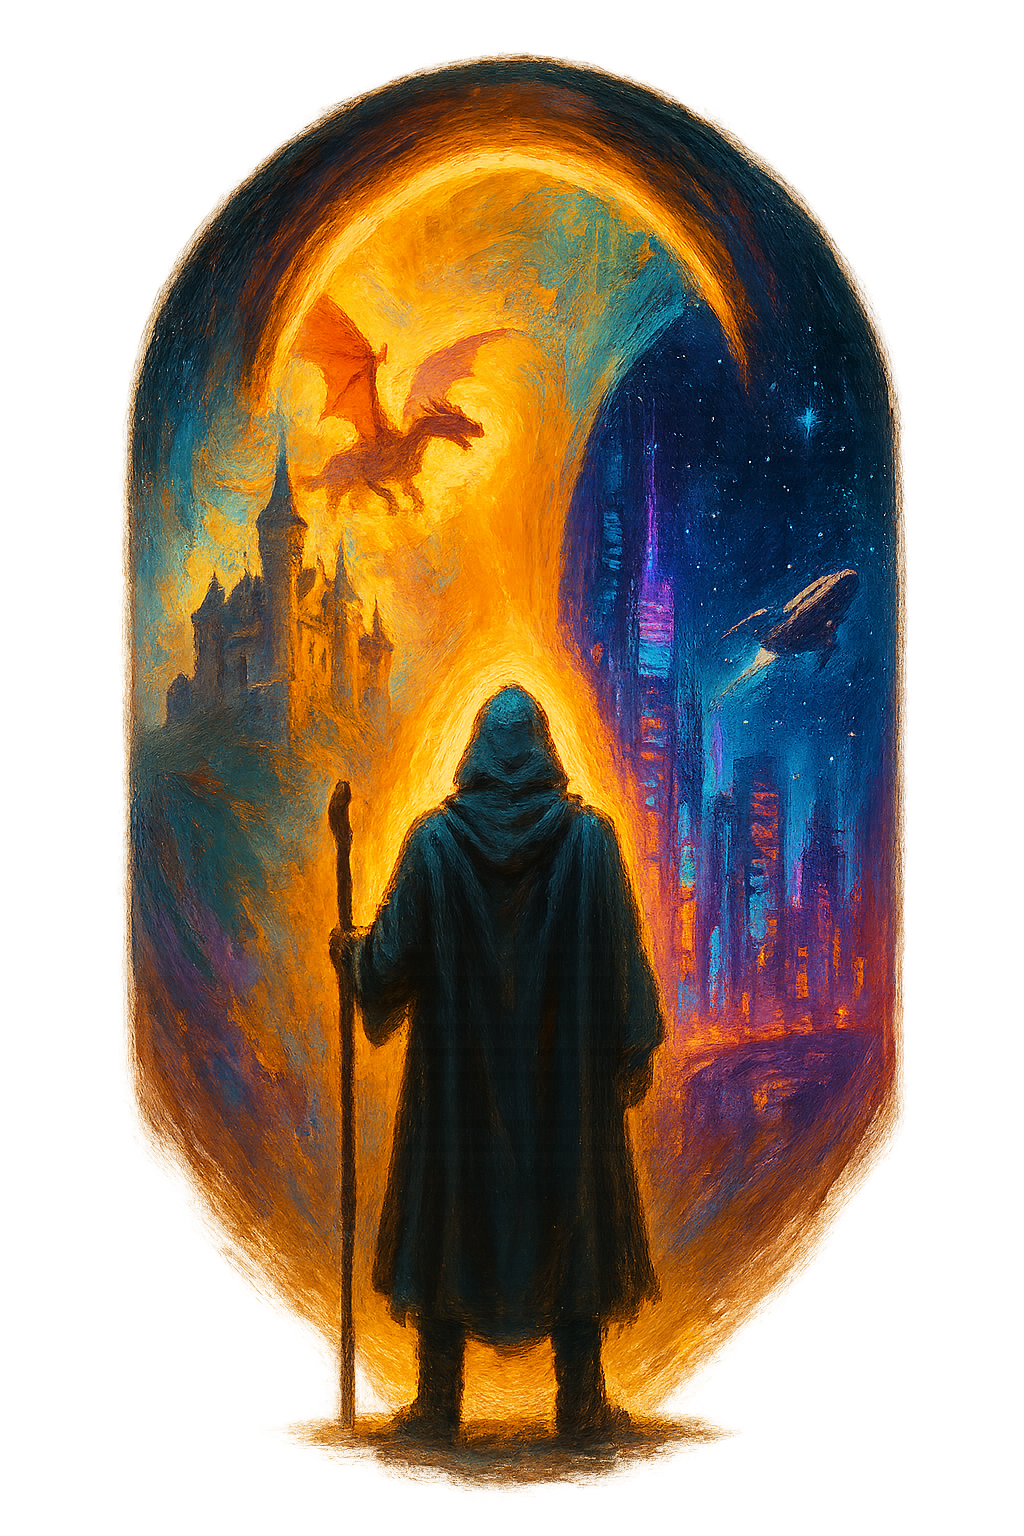
\includegraphics[height=0.5\textheight,keepaspectratio]{art/cover.png}\par
\vspace{\stretch{1}}
{\hdfont\large by Andrew Richardson\par}
\vspace*{\stretch{1}}
\end{titlingpage}

\frontmatter
\tableofcontents

\mainmatter
\twocolumn   % everything after the ToC runs in two columns

% ================================================================
\chapter{Introduction}
% ================================================================
\begin{readaloud}
Every table has its own story. What follows is a system for
telling it --- one set of rules that travels as far as your
imagination will carry it.
\end{readaloud}

\lettrine{L}{egend of the Technomancers} is a tabletop roleplaying
game about travellers who move between worlds. The setting
shifts --- high fantasy one night, rain-slicked cyberpunk the next,
the hard vacuum of deep space the one after that --- but the
characters persist. Their scars, their debts, their hard-won skills:
all of it comes with them. The rules are simple enough to learn
in one session and flexible enough to carry a campaign of a hundred.

One player is the \keyword{Game Master} (GM), who builds the world,
voices its inhabitants, and decides what the dice mean. Everyone
else plays a \keyword{Traveller} --- an exceptional individual
navigating whatever the GM puts in front of them. Travellers are
not superheroes. They are people who have paid attention,
practised hard, and made the choice to step through the wound in
the world when it opened.

\section{What This Game Is About}

At the heart of \emph{Legend of the Technomancers} is a single
question: \emph{what kind of person are you when the world changes?}
The mechanics are built around that question. Your character's
Stats --- \keyword{Body}, \keyword{Mind}, \keyword{Face} --- do not
change when you cross a threshold into a new genre. Your skills
travel with you. Your magic tags re-dress themselves in the
vocabulary of wherever you have landed, but the power behind them
is the same power.

The game rewards players who think about their characters as
\emph{people} first and as stat blocks second. The rules will handle
the numbers. Your job is to decide what your Traveller wants, fears,
and would sacrifice everything for.

\section{How This Book Is Organised}

\begin{itemize}
  \item \keyword{Part I: Building a Traveller} covers character
        creation and a chapter for each of the four columns ---
        Body, Stuff, Skills, and Magic.
  \item \keyword{Part II: Playing the Game} covers the core dice
        engine in full, then the shape of a session: turns, scenes,
        GM tools, and advancement.
  \item \keyword{Part III: The Realms} presents three example
        settings --- High Fantasy, Cyberpunk, and Space Adventure
        --- and shows how the same rules express themselves in
        each one.
\end{itemize}

If you want the short version of how rolls work before diving into
character creation, the core engine is explained in full at the
start of Part~II. The rules in Part~I give you everything you need
to build your Traveller; Part~II explains what to do with them at
the table.

\section{What You Need to Play}

You need a handful of six-sided dice --- a dozen is comfortable,
twenty is luxurious. Every player needs a character sheet (or a
notebook that can serve as one). The GM needs a screen or a
notebook, something to track initiative and hit points behind, and
whatever maps or reference cards feel useful.

Everything else --- imagination, willingness to fail in interesting
ways, a decent snack situation --- you bring yourself.


% ---- Part I: Building a Traveller ----
\part{Building a Traveller}
% ================================================================
\chapter{Character Creation}
% ================================================================
% REAL RULE: four columns, rated 1–4. Keep this.
\lettrine{E}{very character} is described by four columns, each rated on
a scale of \keyword{1 to 4} --- from ordinary to extraordinary: they are
\keyword{Body}, \keyword{Stuff}, \keyword{Skills}, and \keyword{Magic}.
Their meaning bends to fit each realm, but the rank you assign travels
with you from world to world.

\begin{statblock}[The Four Columns at a Glance]
\begin{tabularx}{\linewidth}{@{}p{0.18\linewidth} Y@{}}
\keyword{Body}   & Your physical form --- from ordinary person to dragon.\\[3pt]
\keyword{Stuff}  & What you carry --- from the shirt on your back to a ship.\\[3pt]
\keyword{Skills} & Everything mundane and learned, including combat.\\[3pt]
\keyword{Magic}  & Whatever makes the setting feel fantastic.\\
\end{tabularx}
\end{statblock}

\section{Spending Your Ranks}
% REAL RULE: Shadowrun-style priority. Assign one of A/B/C/D per column.
Character creation borrows the priority method from \emph{Shadowrun}.
You have four priorities --- \keyword{A}, \keyword{B}, \keyword{C}, and
\keyword{D} --- and you assign \emph{one letter to each column}, with no
repeats. \keyword{A} is where you shine; \keyword{D} is where you
struggle. No one is exceptional at everything.

The \keyword{Priority Matrix} on the following page lays out what each
letter means for each column. A priority of \keyword{A} grants the top
rank (\rating{4}) in that column, down to \keyword{D} for the lowest
(\rating{1}).

% ---- Full-width priority matrix: leads a fresh page, then columns resume.
% \twocolumn[<top material>] guarantees flush-top, full-width placement
% (a table* float would centre on a float-only page under memoir).
% NB: no bracketed \\[..] anywhere in this optional arg — a literal ]
% would terminate \twocolumn's [...] early. Use \par + \vspace instead.
\twocolumn[%
  \begingroup\centering
  {\hdfont\Large\bfseries\color{\realmaccent} The Priority Matrix\par}
  \vspace{2pt}
  {\itshape Assign one of A, B, C, D to each column --- one letter each, no repeats.\par}
  \vspace{10pt}
  \endgroup
  \begingroup
  \setlength{\tabcolsep}{7pt}\renewcommand{\arraystretch}{1.35}
  \noindent\begin{tabularx}{\textwidth}{@{}>{\centering\arraybackslash}p{2.3cm} *{4}{Y}@{}}
  \rowcolor{\realmaccent}
  {\hdfont\bfseries\color{white}Priority} &
  {\hdfont\bfseries\color{white}Body}   &
  {\hdfont\bfseries\color{white}Stuff}  &
  {\hdfont\bfseries\color{white}Skills} &
  {\hdfont\bfseries\color{white}Magic}  \\
  \rowcolor{atrBoxbg}
  {\hdfont\LARGE\bfseries\color{\realmaccent}A}\newline\rating{4}
    & Truly strange or monstrous --- a dragon, an angel.
    & A ship, a keep, incredible gear. Rich.
    & A master of many things.
    & A \emph{fucking wizard}; choose 12 tags. \\
  \rowcolor{white}
  {\hdfont\LARGE\bfseries\color{\realmaccent}B}\newline\rating{3}
    & Exceptional --- elven grace, ogrish might, uncanny beauty.
    & A legendary weapon or a vehicle; well off (\$20{,}000).
    & A master of your craft, or a jack of all trades.
    & You know magic; choose 7 tags. \\
  \rowcolor{atrBoxbg}
  {\hdfont\LARGE\bfseries\color{\realmaccent}C}\newline\rating{2}
    & You stand out --- strong, quick, or striking.
    & Ordinary things and some money (\$4{,}000).
    & You know a lot.
    & A few spells; choose 3 tags. \\
  \rowcolor{white}
  {\hdfont\LARGE\bfseries\color{\realmaccent}D}\newline\rating{1}
    & An ordinary person; base stats across the board.
    & Nothing but the shirt on your back.
    & You know a few things.
    & You do not know magic. \\
  \end{tabularx}
  \par\bigskip
  \endgroup
]

\begin{example}
% REAL worked example of the ABCD method.
Mara is a wandering swordmaster who has never touched real magic. She
assigns \keyword{A} to Skills, \keyword{B} to Body, \keyword{C} to Stuff,
and \keyword{D} to Magic.
\end{example}

\section{Stepping Through the Door}
% TODO: how play begins; hand-off to the column chapters.
\lipsum[9]

\begin{notebox}[Design Note: One Sheet, Many Worlds]
% Concept is real (rank travels, meaning is local); prose to be written.
Rank travels but meaning is local, so a single character sheet carries
you across every genre. \lipsum[10][1-3]
\end{notebox}

% ================================================================
\chapter{Body}
% ================================================================
% TODO: opening fiction for Body.
\begin{readaloud}
\lipsum[11][1-3]
\end{readaloud}

\chapterart{col-body.png}

% TODO: what Body means, tone, when it matters.
\lettrine{L}{orem ipsum} \lipsum[12]

% REAL RULE: Body ranks from the Notion source. Keep verbatim.
\begin{statblock}[Body Ranks]
\begin{tabularx}{\linewidth}{@{}p{0.16\linewidth} Y@{}}
\rating{1} & Ordinary person; base stats across the board.\\[3pt]
\rating{2} & Stand out in some way --- strong, quick, or striking.\\[3pt]
\rating{3} & Exceptional --- elven grace, ogrish might, uncanny beauty.\\[3pt]
\rating{4} & Truly strange or monstrous --- a dragon, an angel.\\
\end{tabularx}
\end{statblock}

\section{Body in Play}
% TODO: mechanics/guidance for using Body.
\lipsum[13][1-5]

\section{Changing Shape Across Realms}
% Concept is real: Body keeps its rank but adopts a local form.
\lipsum[14][1-4]

% ================================================================
\chapter{Stuff}
% ================================================================
% TODO: opening fiction for Stuff.
\begin{readaloud}
\lipsum[15][1-3]
\end{readaloud}

\chapterart{col-stuff.png}

% TODO: what Stuff means, tone, when it matters.
\lettrine{L}{orem ipsum} \lipsum[16]

% REAL RULE: Stuff ranks from the Notion source. Keep verbatim.
\begin{statblock}[Stuff Ranks]
\begin{tabularx}{\linewidth}{@{}p{0.16\linewidth} Y@{}}
\rating{1} & Nothing but the shirt on your back.\\[3pt]
\rating{2} & Ordinary things --- armour, a weapon, a skateboard, pocket money.\\[3pt]
\rating{3} & Nice things --- a legendary weapon, a vehicle; generally well off.\\[3pt]
\rating{4} & Amazing things --- a ship, a keep, incredible gear. Rich.\\
\end{tabularx}
\end{statblock}

\section{Stuff in Play}
% TODO: mechanics/guidance for using Stuff.
\lipsum[17][1-5]

\section{Re-Kitting on Arrival}
% Concept is real: translate Stuff into world-appropriate items of same rank.
\lipsum[18][1-4]

% ================================================================
\renewcommand{\realmaccent}{columnSkills}  % forest green
\chapter{Skills}
% ================================================================
% TODO: opening fiction for Skills.
\begin{readaloud}
\lipsum[19][1-3]
\end{readaloud}

\chapterart{col-skills.png}

\lettrine{S}{kills} cover everything mundane and learned --- combat
technique, social grace, technical knowledge, and physical discipline.
Where your Stats describe raw potential, Skills describe what you have
actually practised. A high Agility means you move well; the
\keyword{Blades} skill means you know how to use a sword.

% ---- Section 1: Character Creation ---------------------------------
\section{At Character Creation}

% REAL RULE: Skill ranks from the Notion source. Keep verbatim.
\begin{statblock}[Skill Ranks]
\begin{tabularx}{\linewidth}{@{}p{0.16\linewidth} Y@{}}
\rating{1} & Not very skilful, but you know a few things.\\[3pt]
\rating{2} & You know a lot.\\[3pt]
\rating{3} & A master of your craft, or a jack of all trades.\\[3pt]
\rating{4} & A master of many things.\\
\end{tabularx}
\end{statblock}

Assign one of the four priorities (A through D) to Skills. Your rank
determines the depth and breadth of your training --- how many skills
you know and how good at them you are.

\begin{notebox}[Design Note: Skill Points]
\textbf{To do:} pin down how many skill points each priority grants and
whether any single skill is capped. Working idea: \rating{1} = 4 points,
\rating{2} = 8, \rating{3} = 14, \rating{4} = 20.
\end{notebox}

% ---- Section 2: Rules -----------------------------------------------
\section{Skills in Play}

When you act, choose the skill that covers what you are doing, then pair
it with whichever \keyword{Stat} best fits how you are doing it. The skill
sets the domain; the Stat sets the approach. Roll Stat + Skill dice and
count successes.

\begin{example}
Mara vaults a canyon gap using \keyword{Athletics} + \keyword{Agility}.
She could also talk her way past a guard using \keyword{Persuasion} +
\keyword{Charisma}, or intimidate them with \keyword{Intimidation} +
\keyword{Strength}.
\end{example}

\subsection*{Breadth Versus Depth}
At rank \rating{3} you face a choice: become the undisputed master of one
narrow discipline, or spread your points across a wide range of skills and
know a little about almost everything. Both are valid --- a specialist
punches harder in their lane; a generalist is never completely helpless.

% ---- Section 3: Options ---------------------------------------------
\section{Your Skills}

Each skill entry shows its name, its primary \keyword{Stat}, and a brief
description. The listed Stat is the default pairing; other Stats may apply
if the fiction supports it.

\skillcat{Conflict}
\skill{Blades}{Agility}{Swords, knives, and any weapon that cuts.}
\skill{Brawling}{Strength}{Unarmed combat, holds, and throws.}
\skill{Firearms}{Agility}{Pistols, rifles, and ranged weapons.}
\skill{Archery}{Agility}{Bows, crossbows, and thrown weapons.}

\skillcat{Movement}
\skill{Athletics}{Strength}{Running, climbing, jumping, and swimming.}
\skill{Stealth}{Agility}{Sneaking, hiding, and moving unseen.}
\skill{Piloting}{Agility}{Riding mounts, driving vehicles, and flying craft.}

\skillcat{Social}
\skill{Persuasion}{Charisma}{Convincing others through reason, charm, or appeal.}
\skill{Deception}{Charisma}{Lying, disguise, and misdirection.}
\skill{Intimidation}{Charisma}{Threatening, commanding, and projecting menace.}
\skill{Performance}{Charisma}{Acting, music, and public showmanship.}

\skillcat{Knowledge}
\skill{Lore}{Intellect}{History, legend, culture, and myth.}
\skill{Medicine}{Intellect}{Healing, anatomy, and treating disease.}
\skill{Perception}{Intellect}{Noticing detail, tracking, and reading a scene.}
\skill{Languages}{Intellect}{Speaking, reading, and writing unfamiliar tongues.}

\skillcat{Technical}
\skill{Craft}{Intellect}{Making, repairing, and modifying physical objects.}
\skill{Survival}{Intellect}{Navigation, foraging, shelter, and wilderness living.}
\skill{Hacking}{Intellect}{Electronics, security systems, and information networks.}

% ================================================================
\chapter{Magic}
% ================================================================
% TODO: opening fiction for Magic.
\begin{readaloud}
\lipsum[23][1-3]
\end{readaloud}

\chapterart{col-magic.png}

% REAL (from Notion): "Magic" is whatever makes a setting feel fantastic.
\lettrine{M}{agic} is whatever makes a setting feel fantastic. It is
literal magic in a high-fantasy setting, hacking in a cyberpunk world,
science and engineering in Star Trek, the Force in Star Wars. When you
enter a realm, decide together what Magic \emph{looks like} there.

% TODO: expand on the reskin-per-realm philosophy.
\lipsum[24]

% REAL RULE: Magic ranks from the Notion source. Keep verbatim.
\begin{statblock}[Magic Ranks]
\begin{tabularx}{\linewidth}{@{}p{0.16\linewidth} Y@{}}
\rating{1} & You do not know magic.\\[3pt]
\rating{2} & You can cast a few spells.\\[3pt]
\rating{3} & You know magic.\\[3pt]
\rating{4} & You are a \emph{fucking wizard}.\\
\end{tabularx}
\end{statblock}

\section{Magic in Play}
% TODO: mechanics/guidance for using Magic.
\lipsum[25][1-5]

\section{Reskinning Magic per Realm}
% Concept is real: same rank, different fantastic element per genre.
\lipsum[26][1-4]

% ================================================================
\renewcommand{\realmaccent}{atrAccent}  % reset to default teal
\chapter{Character Advancement}
% ================================================================
% TODO: opening fiction for advancement.
\begin{readaloud}
\lipsum[48][1-3]
\end{readaloud}

\lettrine{C}{haracters} do not advance in the typical way. Instead of
climbing levels, they gain two kinds of points: \keyword{Change Points}
and \keyword{Persistence Points}.

\chapterart[\linewidth]{advance-tattoo.png}

\section{Change Points}
\keyword{Change Points} let you swap one character trait for another of the
same cost. As you travel and grow, who you are can shift --- a tag traded
for a tag, one piece of Stuff for another of equal standing.

\section{Persistence Points}
\keyword{Persistence Points} let you carry some feature forward into other
worlds, exactly as it is in this world.

\begin{example}
Your vehicle is a motorcycle in the 1980s world. Ordinarily it would become
a horse in the fantasy world --- but by spending a Persistence Point you fix
it in its current form forever. When you do, a \keyword{tattoo} appears on
your skin to permanently represent that thing.
\end{example}

\subsection*{How Tattoos Work}
% REAL RULE, 2026-09-22: tattoos are the physical/mechanical marker of a
% spent Persistence Point --- the one thing on the sheet that does NOT
% re-skin between realms. Cross-references the tattoo box on the
% Character Sheet and its "they glow when you spend Persistence Points"
% caption.
Every Persistence Point you spend leaves a mark. The instant you fix
something in place, a new tattoo appears somewhere on your skin ---
permanent ink standing for that one fixed thing, and nothing else. Draw
it yourself, in the tattoo box on your character sheet, as it appears.
By the end of a campaign, your tattoos are a visual record of every
piece of yourself the world was never allowed to take from you.

A tattoo marks the one exception to how everything else on your sheet
works. Your other tags and gear \emph{re-skin} when you cross into a new
realm --- a special weapon becomes a different special weapon, a mount
becomes a motorbike --- but whatever a tattoo represents does not. It
stays exactly as it is, no matter where you go; that permanence is the
whole point of spending the Point.

Tattoos also \keyword{glow} in the instant you spend the Persistence
Point that creates them --- a visible, table-facing signal, for everyone
else at the table, that something has just become permanent. The glow
fades once the moment passes; the ink stays forever.


% ================================================================
\renewcommand{\realmaccent}{atrAccent}  % reset to default teal
\chapter{The Character Sheet}
% ================================================================
% TODO: design and lay out an actual character sheet.
\begin{readaloud}
\lipsum[50][1-3]
\end{readaloud}

\lettrine{Y}{our character sheet} records who this traveller is --- the few
numbers that follow them across every realm, and the truths they carry
within. A finished sheet needs the following elements:

\begin{itemize}
  \item \keyword{Basic attributes} --- the three Stats you roll:
    \begin{itemize}
      \item Body
      \item Mind
      \item Face
    \end{itemize}
  \item \keyword{The four columns} --- what you bought at creation:
    \begin{itemize}
      \item Body
      \item Stuff
      \item Skills
      \item Magic
    \end{itemize}
  \item \keyword{Tattoos} --- features made permanent with Persistence Points.
  \item \keyword{What you know about yourself}.
  \item \keyword{What you have forgotten}.
\end{itemize}



% ---- Part II: The Realms ----
\part{The Realms}
% ================================================================
% Re-theme the realm: emerald accent for High Fantasy.
% (Set BEFORE \chapter so the chapter title is themed too.)
\renewcommand{\realmaccent}{realmFantasy}  % defined in atrpg.sty
\chapter{High Fantasy}
% ================================================================

% TODO: establishing fiction for the fantasy realm.
\begin{readaloud}
\lipsum[27][1-4]
\end{readaloud}

\chapterart{genre-fantasy.png}

% TODO: what this realm is, its tone and tropes.
\lettrine{L}{orem ipsum} \lipsum[28]

\section{Reskinning}
% REAL: this is where the generic catalogue becomes realm-specific.
When you step into High Fantasy, the generic gear on your sheet takes on a
form that fits the realm. A line that simply reads \emph{Mount} becomes a
destrier; a \emph{special weapon} becomes an enchanted blade. Nothing about
your character sheet changes --- only what the entries \emph{look like} here.
The tables below translate each catalogue line into its high-fantasy shape.
Treat them as a starting point: swap in anything of the same rank that suits
your table's vision of the realm.

\subsection{Stuff}
\begin{reskin}{Vehicles}
\reskinrow{Mount \rating{2}}{A warhorse or swift courser --- or, for the bold, an exotic steed: a griffon, a great elk, a dire wolf.}
\reskinrow{Basic Vehicle \rating{3}}{A horse-drawn wagon or coach, a river barge, or a howdah borne on a patient beast of burden.}
\reskinrow{Advanced Vehicle \rating{4}}{A war-chariot, an armoured wagon-fort, or a tamed wyvern that carries you above the field of battle.}
\end{reskin}

\section{Body in High Fantasy}
% TODO: how Body reads here (humans, elves, ogres, dragons...).
\lipsum[29][1-4]

\section{Stuff in High Fantasy}
% TODO: swords, armour, steeds, keeps, legendary artifacts.
\lipsum[30][1-4]

\section{Skills in High Fantasy}
% TODO: swordplay, lore, courtly intrigue, survival.
\lipsum[31][1-4]

\section{Magic in High Fantasy}
% REAL: here, Magic is literal sorcery.
Here, \keyword{Magic} is literal sorcery --- spells, rituals, and the
weave of the arcane. \lipsum[32][1-3]

\begin{notebox}[Running This Realm]
% TODO: GM guidance specific to high fantasy.
\lipsum[33][1-3]
\end{notebox}

\include{chapters/09-cyberpunk}
\include{chapters/10-space-adventure}

\end{document}
